\documentclass[a4j,12pt,]{jarticle}
 \usepackage{float}
 \usepackage{siunitx} %%SI単位系用
 \usepackage{amssymb, amsmath}
 \usepackage{ascmac,here,txfonts}
 \usepackage{hyperref}
 \usepackage{listings}
 \usepackage{pxjahyper}
 \usepackage[dvipdfmx]{graphicx}
 \usepackage{amssymb, amsmath}
  \usepackage{listings}
  \usepackage[dvipdfmx]{color}
 
 \lstset{
   language={Python},
   basicstyle={\ttfamily},
   identifierstyle={\small},
   commentstyle={\small\itshape},
   keywordstyle={\small\bfseries},
   ndkeywordstyle={\small},
   stringstyle={\small\ttfamily},
   frame={single},
   breaklines=true,
   columns=[l]{fullflexible},
   numbers=left,
   xrightmargin=0zw,
   xleftmargin=3zw,
   numberstyle={\scriptsize},
   stepnumber=1,
   numbersep=1zw,
   lineskip=-0.5ex,
 }
\begin{document}

{\noindent\small 第15回報告書 \hfill\today}
\begin{center}
  {\Large ElasticSearchサーバーのデータ移行について}
\end{center}
\begin{flushright}
  祖父江匠真 \\
\end{flushright}

\section{概要}
今回は, 前回に引き続き133.71.106.168から133.71.106.141へのElasticSearchサーバー間のデータ移行とkibanaを用いた可視化結果について報告する.
また, 移行元ElasticSearchサーバーにあったCO\textsubscript{2}データ以外のデータの移行についても報告する.

\section{CO\textsubscript{2}データの移行作業}
前回の報告書では, 移行元ElasticSearchサーバーのCO\textsubscript{2}データについて, JPtimeが2023年より以前のドキュメントを2022\_co2という名前のインデックスに保存し, JPtimeが2023年のドキュメントを2023\_co2という名前のインデックスに保存した.
しかし, インデックスを分けることで2023年以前と2023年のデータをkibanaで同じグラフにプロットして確認することが難しい可能性があることと, ElasticSearchサーバー間のデータ移行が正しく完了したかkibanaで可視化することによって確認することが出来ないという問題があったため, 今回はJPtimeの値に関わらずco2という名前のインデックスに保存した.
保存先のインデックスがco2であることを除くと, データの移行手順は前回のものと同様の手順で行った.

\section{kibanaによるデータの可視化}

移行後のco2インデックスに保存されたデータをkibanaを用いて可視化した.

横軸をタイムスタンプとし, 縦軸をPPM, RH, TEMPとしてそれぞれプロットしたものを図 \ref{p1} 〜 図 \ref{p3}に示す.

\begin{figure}[H]
  \begin{center}
    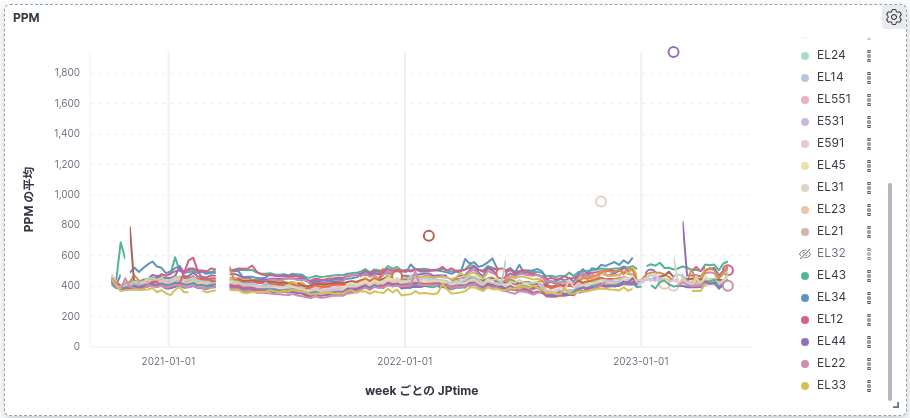
\includegraphics[width=160mm]{ppm.png}
    \caption{co2のPPM}
    \label{p1}
  \end{center}
\end{figure}

\begin{figure}[H]
  \begin{center}
    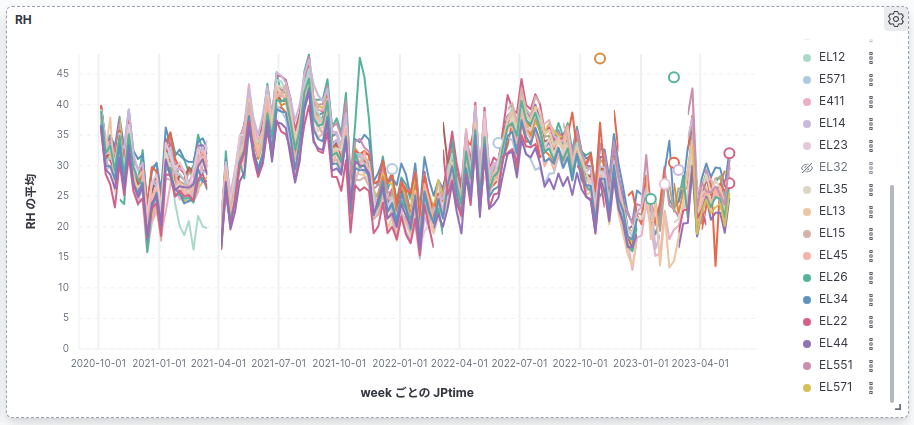
\includegraphics[width=160mm]{rh.png}
    \caption{co2のRH}
    \label{p2}
  \end{center}
\end{figure}

\begin{figure}[H]
  \begin{center}
    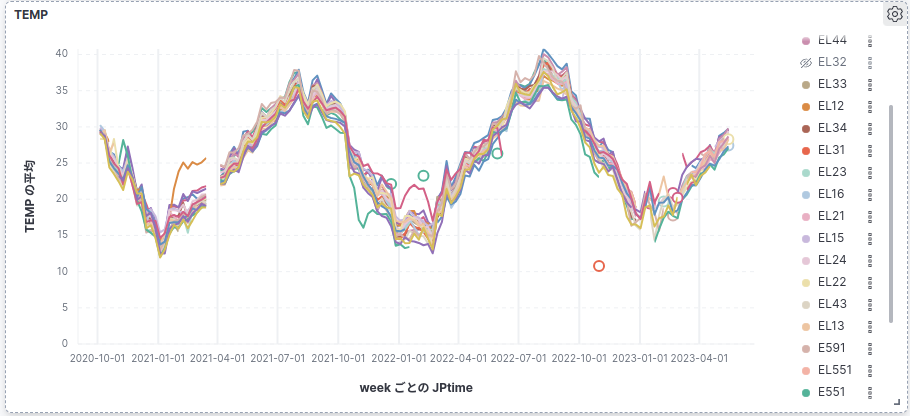
\includegraphics[width=160mm]{temp.png}
    \caption{co2のTEMP}
    \label{p3}
  \end{center}
\end{figure}

図 \ref{p1} 〜 図 \ref{p3}について, 2022年と2023年の境目でデータが連続的に変化していることが確認出来るので, データ移行作業は正常に行うことが出来たと判断できる.

\section{CO\textsubscript{2}データ以外のデータの移行について}

移行元のElasticSearchサーバーにはインデックス名にco2という文字列を含むインデックス以外に以下のインデックスがあった.

\begin{itemize}
  \item movement\_diary
  \item movement\_diary01
  \item temp2
  \item temp3
  \item test
\end{itemize}

これらのインデックスのデータ移行は, 同名のインデックスを移行先のElasticSearchサーバーに作成して, 作成したインデックスにデータを挿入することで行った.

ただし, testインデックスは移行先のElasticSearchサーバーに既に同名のインデックスが作成されていたので, 133.71.106.168\_testというインデックス名にした.

次に, 上記のインデックスに保存されているデータについて説明する.

temp2, temp3はTIME, TEMP, HUMIフィールドを持ったドキュメントが格納されており, temp2のドキュメント数は約150件, temp3は約60件であった.
testはJPtime, PPM, RH, TEMP, ip, number, utctimeフィールドを持ったドキュメントを格納しているインデックスであり, ドキュメント数は95件であった.
これらの情報から, temp2, temp3, testインデックスはCO\textsubscript{2}データの収集の研究の中で動作確認目的に作成されたインデックスではないかと考えられる.

movement\_diaryとmovement\_diary01は運行日誌に関する情報を格納したインデックスであり, それぞれ以下のような構造のドキュメントが保存されている.

\begin{lstlisting}[caption=movement\_diaryのドキュメントデータ, label=sc1]
  {
    "_index": "movement_diary",
    "_type": "_doc",
    "_id": "OL65VHwBr1DnHOWC_d0U",
    "_score": 1.0,
    "_source": {
        "pageNo": "1",
        "type": "運行日誌",
        "wether": "雨",
        "driver": "仲村泰明",
        "passenger": 2,
        "destination": "新田高校・松山聖稜高校",
        "dt_S": "2018-05-08T08:26:00",
        "battery_S": 99,
        "cruisingdistance_S": null,
        "odometer_S": 15,
        "out_charge": "していない",
        "etc": "使用していない",
        "etc_section": "",
        "etc_budget": "",
        "dt_R": "2018-05-08T11:50:00",
        "battery_R": 94,
        "cruisingdistance_AC": null,
        "odometer_R": 30.0,
        "meter": 15.0,
        "start_charg_time": "2018-05-08T11:52:00",
        "remark": "感じなかった",
        "inspection": null,
        "break_rest_Be": null,
        "break_rest_Af": null,
        "tire_rest_Be": null,
        "tire_rest_Af": null,
        "inspection_battery": null,
        "charging_rate": null,
        "health": null
    }
}
\end{lstlisting}

% movement\_diary01は, 基本的にmovement\_diaryと同じフィールド, 同じ値のデータを格納しているが, フィールド"driver"と"destination"の値の型が異なっている.
% movement\_diaryのドキュメントではそれぞれ単一の値を持っているが, movement\_diary01のドキュメントではそれぞれ配列の形式で値が格納されている. また, movement\_diary01のドキュメントにはフィールド "charge\_place", "battery\_rate", "battery\_rate\_distance" が追加されており, "passenger"が削除されている.

\begin{lstlisting}[caption=movement\_diary01のドキュメントデータ, label=sc1]
  {
    "_index": "movement_diary01",
    "_type": "_doc",
    "_id": "oMmqbnwBr1DnHOWCgH9O",
    "_score": 1.0,
    "_source": {
        "pageNo": "1",
        "type": "運行日誌",
        "wether": "雨",
        "driver": [
            "仲村泰明",
            null,
            null
        ],
        "destination": [
            "新田高校",
            "松山聖稜高校"
        ],
        "dt_S": "2018-05-08T08:26:00",
        "battery_S": 99,
        "cruisingdistance_S": null,
        "odometer_S": 15,
        "out_charge": "していない",
        "charge_place": "",
        "etc": "使用していない",
        "etc_section": "",
        "etc_budget": "",
        "dt_R": "2018-05-08T11:50:00",
        "battery_R": 94,
        "cruisingdistance_AC": null,
        "odometer_R": 30.0,
        "meter": 15.0,
        "start_charg_time": "2018-05-08T11:52:00",
        "remark": "感じなかった",
        "inspection": null,
        "break_rest_Be": null,
        "break_rest_Af": null,
        "tire_rest_Be": null,
        "tire_rest_Af": null,
        "inspection_battery": null,
        "charging_rate": null,
        "health": null,
        "battery_rate": 5,
        "battery_rate_distance": 3.0
    }
}
\end{lstlisting}

以下にmovement\_diaryとmovement\_diary01のドキュメントの違いを列挙する.

\begin{enumerate}
\item driverフィールド: 
\begin{itemize}
\item movement\_diaryのドキュメントでは, driverフィールドは文字列である.
\item movement\_diary01のドキュメントでは, driverフィールドは配列で, その中に文字列と2つのnull値が含まれている.
\end{itemize}

\item ``destination''フィールド: 
\begin{itemize}
\item movement\_diaryのドキュメントでは, ``destination''フィールドは単一の文字列である.
\item movement\_diary01のドキュメントでは, ``destination''フィールドは配列で, その中に2つの文字列が含まれている.
\end{itemize}

\item ``charge\_place''フィールド: 
\begin{itemize}
\item movement\_diaryのドキュメントには, ``charge\_place''フィールドは存在しない.
\item movement\_diary01のドキュメントでは, ``charge\_place''フィールドが追加されているが, その値は空文字列である.
\end{itemize}

\item ``battery\_rate''フィールド: 
\begin{itemize}
\item movement\_diaryのドキュメントには, ``battery\_rate''フィールドは存在しない.
\item movement\_diary01のドキュメントでは, ``battery\_rate''フィールドが追加されており, その値は数値である.
\end{itemize}

\item ``battery\_rate\_distance''フィールド: 
\begin{itemize}
\item movement\_diaryのドキュメントには, ``battery\_rate\_distance''フィールドは存在しない.
\item movement\_diary01のドキュメントでは, ``battery\_rate\_distance''フィールドが追加されており, その値は数値である.
\end{itemize}

\end{enumerate}

\section{まとめ}
今回は, ElasticSearchサーバー間でのデータ移行とkibanaを用いた可視化結果について報告した.
すべてのCO\textsubscript{2}データをco2という名前のインデックスに格納してkibanaで可視化した結果, 2022年と2023年の境目でデータが連続的に変化していることが確認出来たので, データ移行は正しく行えたと判断した.

また, 移行元ElasticSearchサーバーにあったインデックス名にco2を含まないインデックスの移行作業についても報告した.

\end{document}